\def\iangle{35} % Angle of the inclined plane
\def\down{-90}
\def\arcr{0.5cm} % Radius of the arc used to indicate angles


\def\lengthVector{1.5}

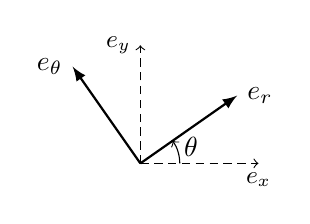
\begin{tikzpicture}[
    axis/.style={densely dashed, font=\small},
]
        
    \draw [->,axis] (0,0) coordinate (O) -- ++(\lengthVector,0) node [below] {$\vv{e_x}$};
    \draw [->,axis] (O) --++ (0,\lengthVector) node [left] {$\vv{e_y}$};
    
    \draw [->,>=latex, thick] (O) -- ++(\iangle:\lengthVector) node [right] {$\vv{e_r}$};
    \draw [->,>=latex, thick] (O) -- ++(\iangle+90:\lengthVector) node [left] {$\vv{e_\theta}$};
    
    \draw[->] (O)++(\arcr,0) arc (0:\iangle:\arcr);
    \path (O)++(\iangle*0.5:\arcr+5pt) node {$\theta$};
\end{tikzpicture}
